%!TEX root = ../BoYu-Dissertation.tex
\graphicspath{{Figures/}}

\chapter{Introduction} 
\label{chapter1:introduction}

\section{Problem scope}
\label{sec:problem_scope}
Awareness is one of the most active research areas in computer supported cooperative work (CSCW) \cite{dourish1992awareness,schmidt2002a,rittenbruch2009a}. At its essence, awareness refers to the ability of collaborators to understand each other's activities and relate them to a joint context \cite{rittenbruch2009a}. This context is essential for collaboration as it is used to ensure that individual contributions are relevant to the group's activity as a whole, and allow groups to coordinate the process of collaborative work \cite{dourish1992awareness}. 

Awareness falls into the category of `articulation work' that is required for collaborative work but not its primary goals \cite{schmidt1992taking}. People want to maintain the awareness of one another to ensure their joint effort is coordinated and integrated, but at the same time they want to do it effortlessly so that it does not interrupt their current line of work \cite{fussell1998coordination}. This is unproblematic in ordinary face-to-face environments where the mechanics of collaboration are natural, spontaneous, and unforced \cite{Gutwin2002}. However, it becomes a significant task in distributed collaboration because of the limited interaction resources available to the actors \cite{carroll2003a}. As a result, a large number of computer-supported awareness mechanisms and tools have been proposed in the literature, aiming to support awareness in distributed collaboration with minimal attention and effort from the participants of teamwork \cite{rittenbruch2009a,markopoulos2009design}.

Although much progress has been made in designing awareness mechanisms to support distributed collaboration at relatively small and medium scales \cite{antunes2010a}, it becomes a much more difficult task to support awareness in complex and highly distributed activities \cite{cabitza2009promoting}. The collaborative activities of interest in this study are these large-scale distributed collaborative settings, where awareness is unlikely to be achieved effortlessly, and hence it becomes even more important to design computational artifacts to support awareness. In the rest of this section, we first define the scope of large-scale collaborative environments in this study, and then present the major challenges for awareness support in these environments that motivate this work.

\subsection{Large-scale collaboration} % (fold)
\label{sub:complex_collaboration}
In general, collaborative activities we consider in this study are a subset of synchronous and distributed collaborative settings \cite{Ellis1991}, with a higher level of complexity and dynamics:

\begin{enumerate}
\item \emph{Higher level of complexity}: The collaborative activities in this study usually include a large number of team workers that engage in a variety of distributed, yet interdependent actions. On one hand, the collaborators play specialized roles, possess distinct knowledge, and perform different actions in the course of joint endeavors. On the other hand, their actions are inter-connected because of a variety of dependencies that may occur. 

\item \emph{Higher level of dynamics}: The actors work in dynamic settings that entail frequent changes in the environment and their activities. As a result, plans of the collaborative activities are under continuous development and the tasks and roles of team members cannot be precisely specified in advance.
\end{enumerate}

Examples of large-scale collaboration within these boundaries abound in practical applications such as emergency response \cite{Turoff2004}, medical systems \cite{Blandford2004}, and military training \cite{mathieu2000influence}. Our interest in supporting awareness is motivated by the need to support large-scale distributed collaboration in emergency response operations \cite{Cai2005b,Cai2005a}. An example of these collaborative environments under discussion can be illustrated in the following scenario.

\begin{scenario}
\textbf{An Emergency Response Scenario.} 
Due to a critical accident in a nuclear plant, a large quantity of radioactive substance is accidentally released in the atmosphere. To respond to this critical incident, task force is formed that includes search and rescue teams, decontamination teams, medical treatment teams, and transportation teams. Teams are dispatched and configured geographically to cover the impacted area. Each team covers a functional area of the overall mission.  Search and rescue teams patrol the incident area to search for victims and report their locations and status. Discovered victims are first decontaminated (by one of the decontamination teams) before they can be moved to other facilities.  If a victim is wounded, he or she will be scheduled and transported to a medical station for treatment. All transportation needs for moving victims to treatment stations and shelters are handled by the transportation team. Although teams are working autonomously on their local tasks, they must coordinate their capacity, schedule, and priority to deal with emerging and unexpected situations in order to save and protect all the victims in an efficient fashion.
\end{scenario}

Such an emergency situation usually involves multiple individuals and organizations that are distributed in different geographic locations (emergency operation center, mobile command-and-control posts, medical stations, etc.). The different actors have complementary knowledge and skills, and hence divide the work so that they can work relatively autonomously within their local environment and responsibilities. In the same time, actions of different actors are interleaved with each other due to different types of dependencies \cite{shen2004managing}. For example, the decontamination action can only be performed after the victim is transported to the station, and the medical treatment can only be performed after the victim is decontaminated.

Furthermore, exceptions to the planned responses are a common and critical factor in these activities \cite{Turoff2004}. Re-planning of actions and re-allocation of resources go on as a continuous unpredictable process. When a rescue vehicle breaks down, it creates a limitation on the use of the vehicle to transport the victim, which leads to the assignment of another vehicle to the action, or even re-planning of the whole activity to rescue the victim. In such dynamic environment, what specific information is of concern and interest to a given individual is changing rapidly.
% subsection complex_collaboration (end)

\subsection{Challenges in awareness support} % (fold)
\label{sub:challenges_in_awareness_support}
The increased level of complexity and dynamics in these collaborative environments poses major design challenges for awareness support, which have limited support in existing awareness supporting systems.

\paragraph*{Managing increased level of complexity} % (fold)
\label{par:managing_increased_level_of_complexity}
With low level of complexity, awareness can be achieved by means of presenting `shared spaces' among collaborators. This can be `shared media spaces' that provide continually audio-video links between distributed actors \cite{Dourish1992}, or `shared virtual spaces' that provide various types of virtual spaces to support awareness, such as virtual meeting rooms \cite{Berlage1999}, or more popularly, `shared workspaces' where people can see and manipulate artifacts related to their activities \cite{Gutwin2002}. Despite the different forms `shared spaces' can take, they have the same goal to make the shared work settings visible, so that people can keep an eye on what the rest of the group is doing while doing their individual work, and develop the shared awareness of the group situation \cite{schmidt2002a}.

However, when the complexity of the collaborative activities scales up, maintaining a shared understanding of the whole situation becomes more difficult, and less desired by the team members. First, the magnitude of the collaborative work can grow significantly as hundreds or thousands of actors engage in myriads of interdependent activities. It becomes difficult or even impossible to share all the aspects in the field of the collaborative work with every actor. Furthermore, these complex activities are usually highly distributed as team members play specialized roles and engage in different actions. Team members experience the situation in different ways, as defined by their own personal goals, roles, tasks, skills, and so on. Team members have their own awareness, related to the goals that they are working towards. Even though they may have access to the same information, differences in goals, roles, the tasks being performed make them view it differently \cite{Salmon2010}. As a result, it becomes more important for the awareness system to understand and support team members' distinct awareness requirements, rather than merely making the shared context visible.
% paragraph managing_increased_level_of_complexity (end)

\paragraph*{Handling increased level of dynamics} % (fold)
\label{par:handling_increased_level_of_dynamics}
Developing appropriate awareness mechanisms must be based on a solid understanding of the team members' awareness requirements, e.g. what kinds of awareness information is relevant to each team member, or how the information should be presented. In relatively static work domains, the set of awareness requirements can be identified in advance so that the awareness system can be designed to support them. However, in these dynamic environments characterized by frequent and continuous changes in the environment and activities, team members' awareness requirements are quite fleeting. In order to adapt to these changes, the actors engage in different actions, assign and reassign resources for them, or change their ways to perform them. As the collaborative activity develops, they are likely to modify their awareness requirements accordingly to achieve their changing goals. As a result, it would be highly desirable for the awareness systems to be able to keep track of these dynamics over time and assess the actors' changing awareness requirements as they emerge in the evolving collaborative activities.
% paragraph handling_increased_level_of_dynamics (end)
% subsection challenges_in_awareness_support (end)
% section problem_scope (end)

\section{Research approach and contributions} % (fold)
\label{sec:research_approach_and_contributions}
By setting the scene in the previous section, the overall objective of this dissertation is to address the major challenges of awareness support as distributed collaborative activities are scaled up to more complex and dynamic situations. To achieve the research objective, this study follows the design science paradigm in information systems research \cite{Hevner2004}. Knowledge and understanding of the aforementioned awareness problems in large-scale collaboration and their solutions are achieved through a set of design activities to develop useful and usable awareness supporting systems. Figure \ref{fig:research_overview} provides the overview of the research approach in this study.

\begin{figure}[htbp] %  figure placement: here, top, bottom, or page
   \centering
   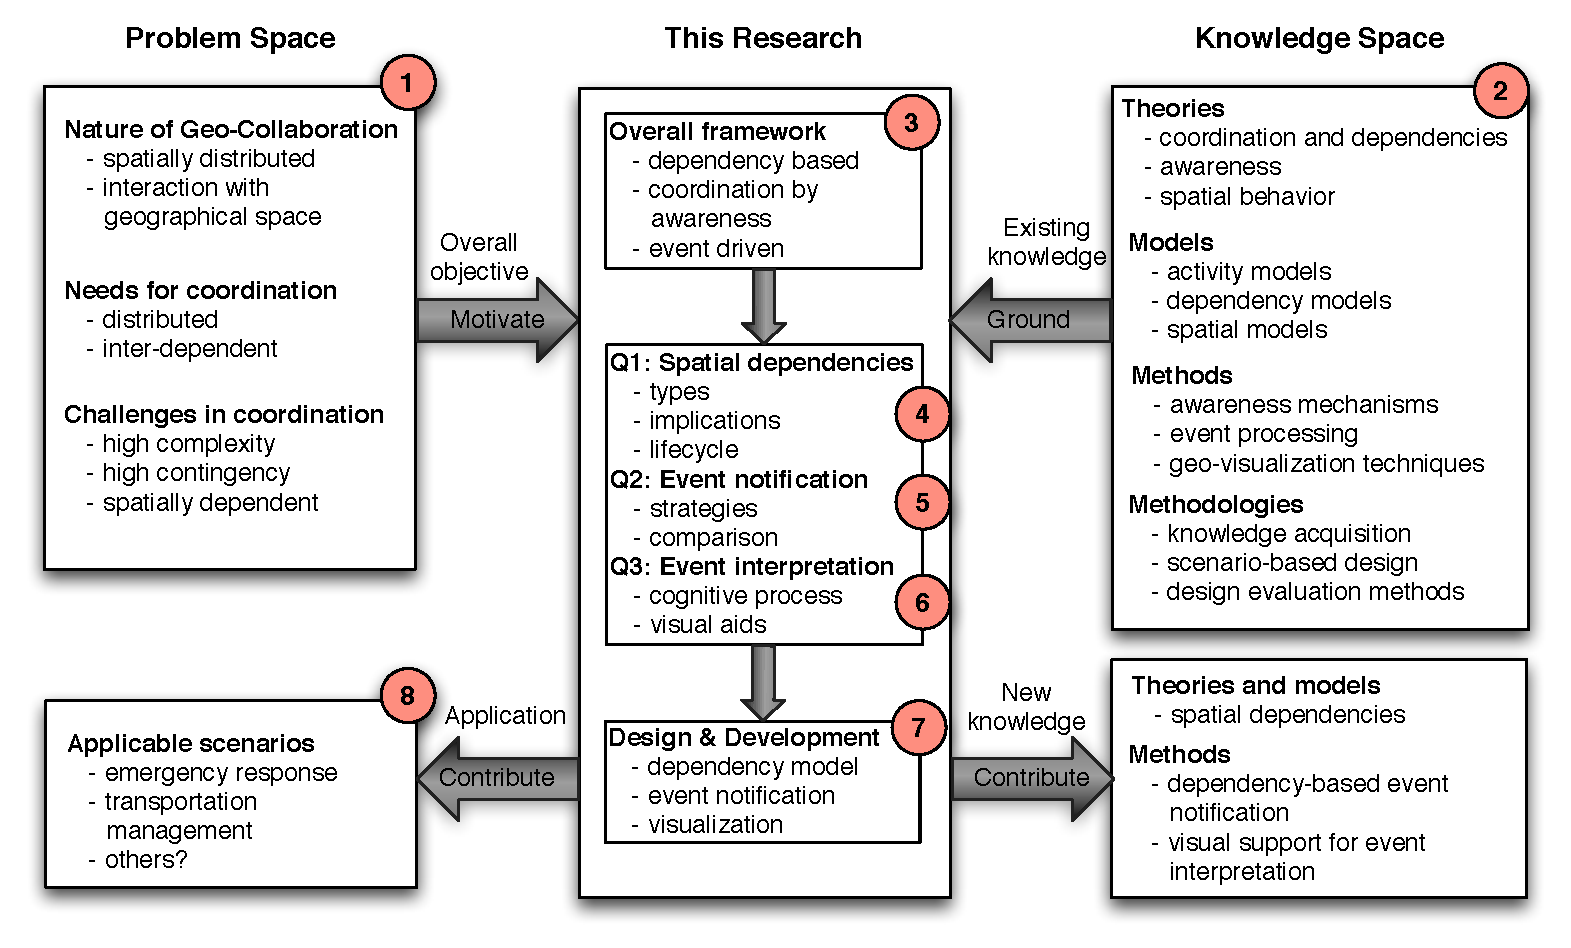
\includegraphics[width=5.8in]{research_overview.pdf} 
   \caption{Overview of the research approach}
   \label{fig:research_overview}
\end{figure}

The research starts with defining the problem scope and specifying the design challenges in the problem scope (Chapter \ref{chapter1:introduction}). Then existing knowledge about theories and models to understand the awareness phenomena is reviewed to provide the theoretical foundation of this study (Chapter \ref{cha:understanding_awareness}). Based on the grounding work in the literature, we develop the conceptual model to understand the awareness phenomena in large-scale distributed collaboration (Chapter \ref{cha:the_conceptual_framework}). Such a conceptual model helps us to develop concrete design issues that need to be addressed, identify knowledge gaps in existing studies, and guide our design of the computational awareness promotion framework (Chapter \ref{cha:awareness_promotion}, \ref{cha:knowledge_reprsentation_and_updating}, and \ref{cha:promoting_event_driven_awareness}). Following the computational approach, we develop the prototype system to prove the feasibility of the approach (Chapter \ref{cha:system_implementation}). Then we perform the case study in a concrete emergency response scenario to demonstrate the utility of our approach in supporting awareness in large-scale distributed collaboration (Chapter \ref{cha:case_studies}). 

Following the design-research paradigm, the contributions of this research can be analyzed from two aspects: (1) the development of theories or models that extend and improve the understanding of design problems, (2) and the development of methods or tools that enable solutions to the design problems (Chapter \ref{cha:conclusion}). More specifically, this study contributes to awareness support in collaborative activities at two levels:

\begin{enumerate}
	\item First, we provide an integrated conceptual model for understanding the awareness phenomena in large-scale distributed collaborations. Our conceptual model is built on top of existing theories and models, and in turn contribute to existing knowledge foundations in two aspects: (1) We emphasize the distributed nature of the awareness phenomena, i.e. each team member's awareness is partial, but at the same time is compatible for the team to perform the collaborative activity successfully. (2) Our model provides a better explanation of how the compatibility of different collaborators' awareness is achieved through the integration of individual cognitive processes and social processes.
	\item The second major contribution of this study is the computational awareness promotion approach that aims to design a knowledge-based awareness system that maintains a collective knowledge representation of the collaborative work, and utilizes it to support the various awareness processes. With the help of the formal knowledge representation, the awareness promotion approach shows several advantages to handle the scaled up complexity and dynamics in collaborative activities, and provides integrated awareness support.
\end{enumerate}
% section research_approach_and_contributions (end)